\chapter{Graph Tracking in Probabilistic Models}
\label{cha:graph-track-prob}

The system described in chapter~\ref{cha:impl-dynam-graph}, implemented in a Julia package
\irtrackerjl{}, can now be utilized for the analysis of probabilistic models written in \dppljl{},
and for posterior inference in \turingjl{}.  This part of the work is realized in another package,
\autogibbsjl{}, which is available as open-source
code\footnote{\url{https://github.com/phipsgabler/AutoGibbs.jl}}.  There are two applications
provided, built on top of the graph tracking functionality: first, dependency analysis of random
variables in a model can be performed.  This results in the complete graphical model for static
models, and a slice of it for dynamic models.  The resulting graph can be plotted for visualization.
Second, given the dependency graph, the conditional likelihoods of unobserved variables in static
models can be extracted.  With these, analytic Gibbs conditionals can be derived and used in
\turingjl{}'s within-Gibbs sampler.

\section{Dependency Analysis in Dynamic Models}
\label{sec:dependency-analysis}

In order to use \irtrackerjl{} to extract the dependencies in a probabilistic model written in
\dppljl{}, we need to remember the structure of such models, which was introduced in
section~\ref{sec:prob-prog}: there is one evaluator function, into which the original code is
transformed, and which evaluates the model in different modes.  This function has the same structure
as the original code, but adds some more complicated book-keeping logic to it, and transforms the
tilde statements into function calls with some additional metadata.  Furthermore, when calling the
model as a callable object, there are several layers of dispatch (about five layers of nesting),
until the real evaluator function is actually hit.  On the other hand, there is no further nesting
involved beyond the evaluator function~-- \turingjl{} simply does not support nested models, for
technical reasons.

Therefore, we at first need to introduce an \irtrackerjl{} context that will record all the internal
function calls down to the evaluator function, and stop there.  Similar to the
\jlinl{DepthLimitContext} demonstrated on page~\pageref{lst:depthlimitcontext}, the main task here
is to overload the \jlinl{canrecur} method to stop at the right call.  This can easily be done by
introducing a helper predicate function \jlinl{ismodelcall} that dispatches on the involved types.
Next, we notice that the resulting computation graph consists of a nested and quite unusable
structure, due to the initial levels of nesting.  To work with it the model code, we need to strip
the outer layers off the inner node containing the trace of the evaluator function.  Thirdly, many
of the statements in the trace of the evaluator function do not have relevance for dependency
analysis~-- like those that stem from internal calculations done by the model, or statements that
were written by the user but to not lie on the dependency graph, such as debugging statements or the
lowered code of for loops, in some cases.  These we can strip off in advance, so as to clean the raw
dependency trace.  These three preparation steps are put together in one method:
\begin{lstlisting}
function slicedependencies(model::Model{F}, args...) where {F}
    trace = trackmodel(model, args...)
    strip = strip_model_layers(F, trace)
    slice = strip_dependencies(strip)
    return slice
end
\end{lstlisting}
Here, \jlinl{trackmodel} extracts the computation graph with the context for models tracking,
\jlinl{strip_model_layers} removes the outer method calls, and \jlinl{strip_dependencies} removes
all SSA code that is not on the dependecy graph spanned by the sampling statements.

The final and most intricate step is to add all the remaining SSA statements to a new graph
structure, that describes a more domain-specific representation.  In this \jlinl{Graph} type, only
assumption, observation, call, and constant nodes remain, containing relevant metadata such as their
values, variable names, and distribution objects.  In addition, the object stores intermediate
information used during its construction, such as the mapping between newly generated and original
references.  The graph construction is implemented in a function \jlinl{makegraph}, and we finally
have one exported function
\begin{lstlisting}
function trackdependencies(model, args...)
    slice = slicedependencies(model, args...)
    return makegraph(slice)
end
\end{lstlisting}
There are two complications regarding \jlinl{makegraph}.  For one, model arguments are handled
specially by \dppljl{}~-- there are some internal arguments added, and the original arguments are
inspected to allow to run the same model in generative or posterior mode.  This part needs to be
sorted out, so that the passed argument values are correctly set up as constants in the dependency
graph, but since all information is present, the task is resolved by correctly identifying the
arguments and restructuring their contents into the right form.

The other problem is the handling of mutation, and tracking of modified array elements.  For
example, a hidden Markov model might contain code like this:
\begin{lstlisting}
s = zeros(Int, N)
s[1] ~ Categorical(K)
for i = 2:N
    s[i] ~ Categorical(T[s[i-1]])
end
\end{lstlisting}
In order to express the dependency between successive elements of \jlinl{s}, an empty array is first
set up, and then subsequently populated by the results of the tilde statements describing the Markov
process.  In this form, only the individual variables \jlinl{s[i]} are recognized by the model
language.  Internally, the tilde statements are translated to array assignments of the form
\jlinl{s[i] = tilde_assume(...)}, but with additional lowering of the involved arguments, after
which the corresponding IR will look approximately like this:
\begin{lstlisting}
%9 = %i - 1                 # i - 1
%10 = getindex(%s, %9)      # s[i - 1]
%11 = getindex(%T, %10)     # T[s[i - 1]]
%12 = VarInfo{:s}(((%i,),))
%13 = Categorical(%11)
%14 = tilde_assume(..., %13, ..., %12, ...)
%15 = setindex!(%a, %14)
\end{lstlisting}
(to be understood symbolically, not as real SSA~-- several statements have been collapsed).  We see
that the direct association between the variable \jlinl{s} is not preserved in the line of the tilde
method, but spread over multiple statements. Even worse, since all statements for the different
\jlinl{s[i]} result in mutations of \jlinl{\%a}, the immediate dependency between \jlinl{s[i]} and
\jlinl{s[i-1]} is not available as a data dependency, but must be recovered dynamically.

The \jlinl{makegraph} implementation solves this by successively identifying mutated arrays
representing random variables by inspecting the indexing calls around tilde statements, and storing
the association between the assumption and the array elements.  This part of the procedure is the
most intricate one, and not complete; there may exist cases where mutation is able to
\enquote{circumvent} the dependecy analysis.  Additionally, the matching between indexing arguments
involves some careful treatment of variable names; the existing \dppljl{} API for this functionality
is not very comprehensive.

Due to this, the current implementation of \autogibbsjl{} currently only supports \enquote{simple}
indexing by one tuple of integers.  Other, more general indexing styles allowed in Julia could be
added in future extensions.  Furthermore, broadcasting tilde statements, that are supported in
\dppljl{}, are not supported by \autogibbsjl{} either.

\newthought{As an example} for the resulting graphs, take the two simple models in
listing~\ref{lst:dependency-examples}.  The pretty-printed dependency \jlinl{Graph}s of them are
shown in listing~\ref{lst:trace-examples} below.  We can see that the model arguments for
observations occur as constant values, and all of the intermediate transformation visible in the
original model definitions are observed.  From this structure, \autogibbsjl{} can construct output
in the Dot graph format and vizualized using GraphViz \parencite{gansner2000open}.  The visual
outputs of the example models is shown in figure~\ref{fig:geom-deps}.

\begin{lstfloat}[p]
\begin{lstlisting}[style=lstfloat]
@model function bernoulli_mixture(x)
    w ~ Dirichlet(2, 1/2)
    p ~ DiscreteNonParametric([0.3, 0.7], w)
    x ~ Bernoulli(p)
end

@model function hierarchical_gaussian(x)
    λ ~ Gamma(2.0, inv(3.0))
    m ~ Normal(0, sqrt(1 / λ))
    x ~ Normal(m, sqrt(1 / λ))
end
\end{lstlisting}
  \caption{Two simple example models: a mixture of two Bernoulli random variables with fixed
    probabilities, and a Gaussian model with conjugate prior.  Both models are defined over one
    single observation.}
  \label{lst:dependency-examples}
\end{lstfloat}

\newsavebox{\bernoullitrace}
\begin{lrbox}{\bernoullitrace}
\begin{lstlisting}[style=lstfloat]
⟨2⟩ = false
⟨3⟩ = Dirichlet(2, 0.5) → Dirichlet{Float64}(alpha=[0.5, 0.5])
⟨4⟩ = w ~ ⟨3⟩ → [0.826304431175434, 0.17369556882456608]
⟨5⟩ = DiscreteNonParametric([0.3, 0.7], ⟨4⟩) → DiscreteNonParametric{...}(
        support=[0.3, 0.7], p=[0.826304431175434, 0.17369556882456608])
⟨6⟩ = p ~ ⟨5⟩ → 0.3
⟨7⟩ = Bernoulli(⟨6⟩) → Bernoulli{Float64}(p=0.3)
⟨8⟩ = x ~ ⟨7⟩ ← ⟨2⟩
\end{lstlisting}
\end{lrbox}
\newsavebox{\gaussiantrace}
\begin{lrbox}{\gaussiantrace}
\begin{lstlisting}[style=lstfloat]
⟨2⟩ = 1.4
⟨3⟩ = Gamma(2.0, 0.3333333333333333) → Gamma{Float64}(
        α=2.0, θ=0.3333333333333333)
⟨4⟩ = λ ~ ⟨3⟩ → 0.9257859525673857
⟨5⟩ = /(1, ⟨4⟩) → 1.0801632896100921
⟨6⟩ = sqrt(⟨5⟩) → 1.0393090443222806
⟨7⟩ = Normal(0, ⟨6⟩) → Normal{Float64}(μ=0.0, σ=1.0393090443222806)
⟨8⟩ = m ~ ⟨7⟩ → 1.8505166567138398
⟨9⟩ = /(1, ⟨4⟩) → 1.0801632896100921
⟨10⟩ = sqrt(⟨9⟩) → 1.0393090443222806
⟨11⟩ = Normal(⟨8⟩, ⟨10⟩) → Normal{Float64}(
         μ=1.8505166567138398, σ=1.0393090443222806)
⟨12⟩ = x ~ ⟨11⟩ ← ⟨2⟩
\end{lstlisting}
\end{lrbox}
\begin{lstfloat}[p]
  \loosesubcaptions
  \subbottom[Trace of \texttt{bernoulli\_mixture(false)} (some type parameters not shown).]{%
    \usebox{\bernoullitrace}}
  \subbottom[Trace of \texttt{hierarchical\_gaussian(1.4)}.]{%
    \usebox{\gaussiantrace}}
  \caption{Traced structure of the two example models introduced above.  Values in \(\langle\)angle
    brackets\(\rangle\) denote intermediate values (similar to SSA variables), and right arrows
    denote the resulting values of function calls.  The left arrow indicates the source of the
    observed value.}
  \label{lst:trace-examples}
\end{lstfloat}

\FloatBlock

\begin{figure}[p]
  \centering
  \subbottom[][\texttt{bernoulli\_mixture(false)}]{%
    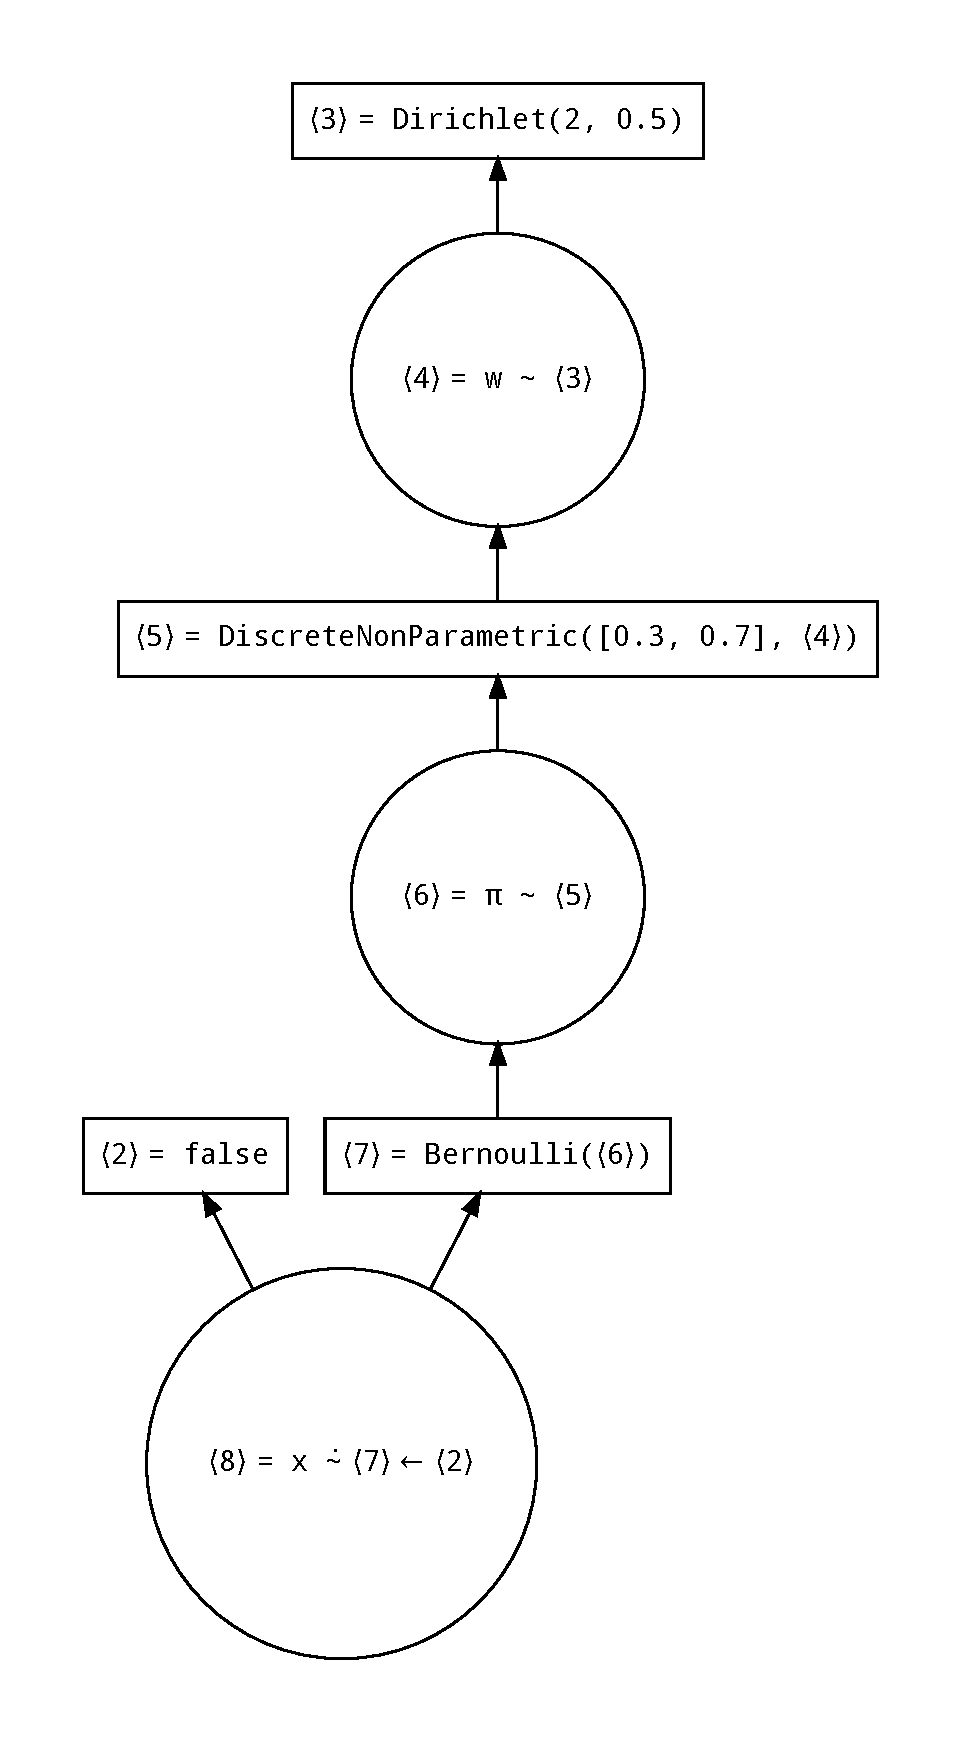
\includegraphics[width=0.49\textwidth]{figures/bernoulli_dependencies}}
  \subbottom[][\texttt{hierarchical\_gaussian(1.4)}]{%
    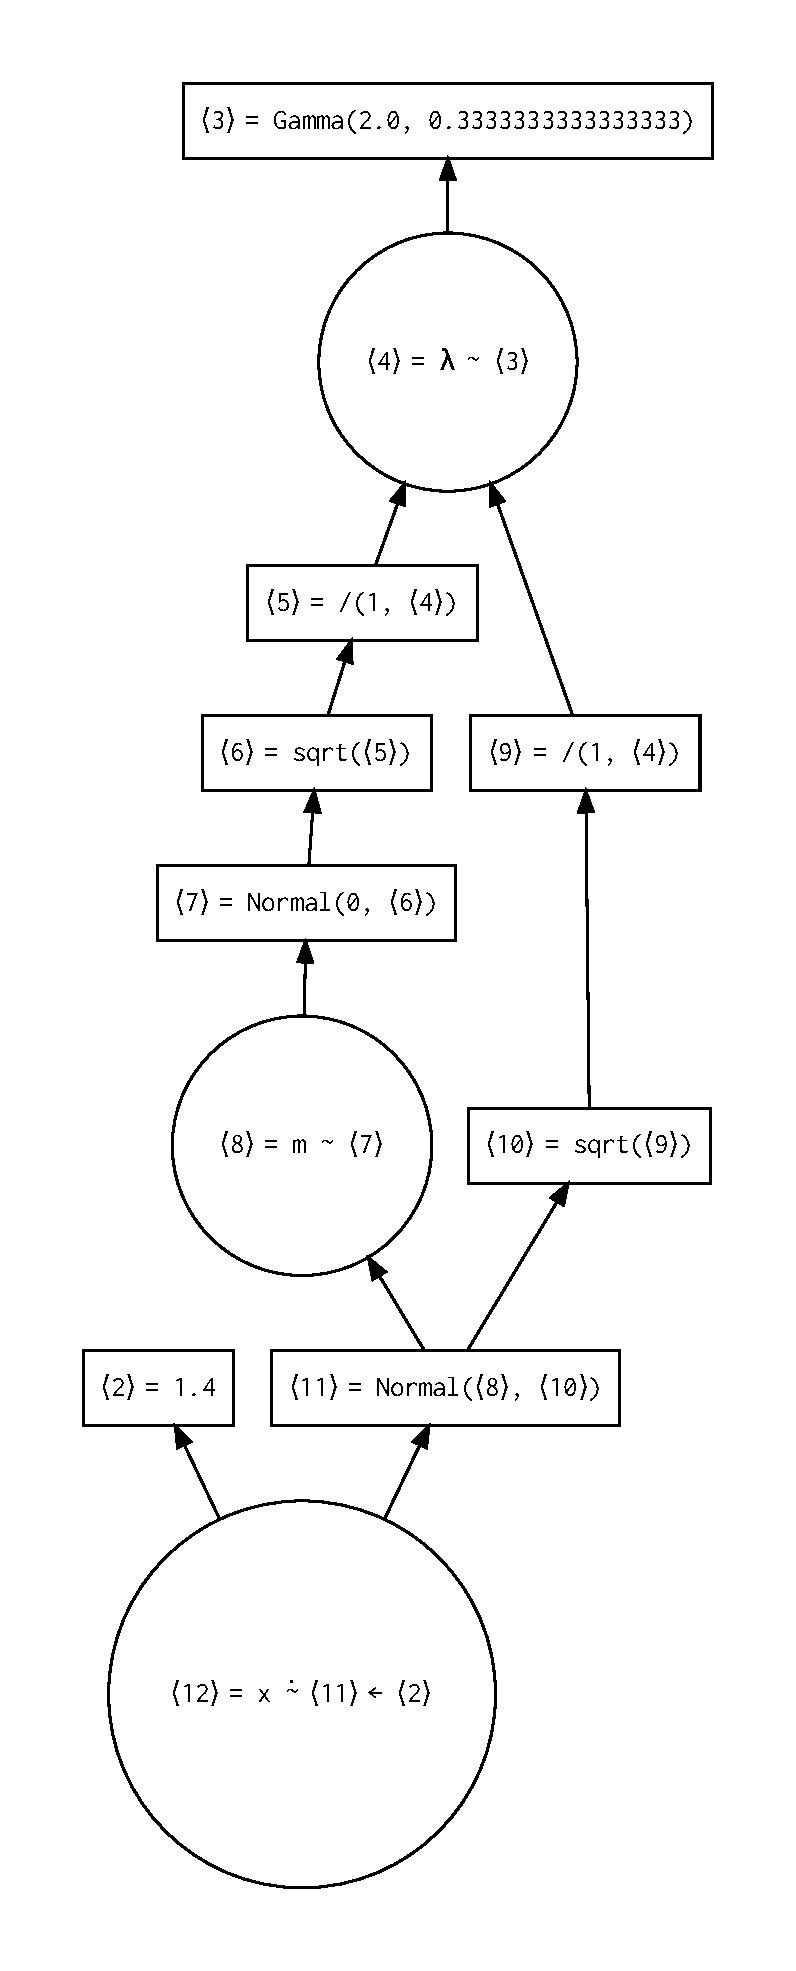
\includegraphics[width=0.49\textwidth]{figures/gaussian_dependencies}}
  \caption{Dependency graphs of the models in listing~\ref{lst:dependency-examples}, generated by
    \autogibbsjl{} and rendered by GraphViz.  More information, such as node values, is stored in
    the real model graph, but not printed for better readability.  Circular nodes denote tilde
    statements, while deterministic intermediate values, corresponding to normal SSA statements, are
    written in rectangles.}
  \label{fig:geom-deps}
\end{figure}


\section{JAGS-Style Automatic Calculation of Gibbs Conditionals}
\label{sec:jags-style-conditionals}

Gibbs sampler implementation for Turing; likelihood closures; conditional likelihood extraction


\section{Evaluation}
\label{sec:autogibbs-eval}

\begin{table}[t]
  \centering
  \libertineTabular
  \begin{tabularx}{\textwidth}{XXrrr@{\hskip 10mm}rrrr}
    \toprule
     & & \multicolumn{3}{c@{\hskip 10mm}}{\textbf{GMM}} & \multicolumn{3}{c}{\textbf{HMM}} & \multicolumn{1}{c}{\textbf{IMM}} \\
    \midrule
    & HMC Steps & & 10 & & & 10 & & 10 \\
    & HMC Step size & & 0.1 & & & 0.1 & & 0.1 \\
    \midrule
    \textbf{AG + HMC} & Data size & 10 & 25 & 50 & 10 & 25 & 50 & 10 \\
    & Chains & 30 & 30 & 30 & 30 & 30 & 30 & 30 \\
    & Compilations & 3 & 3 & 3 & 3 & 3 & 3 & 3 \\
    \addlinespace
    \textbf{PG + HMC,} & Data size & 10 & 25 & 50 & 10 & 25 & 50 & 10 \\
    \textbf{10 particles} & Chains & 10 & 10 & 10 & 10 & 10 & 10 & 10 \\
    \addlinespace
    \textbf{PG + HMC,} & Data size & 10 & 25 & 50 & 10 & 25 & 50 & 10 \\
    \textbf{25 particles} & Chains & 10 & 10 & 10 & 10 & 10 & 10 & 10 \\
    \addlinespace
    \textbf{PG + HMC,} & Data size & 10 & 25 & 50 & 10 & 25 & 50 & 10 \\
    \textbf{50 particles} & Chains & 10 & 10 & 10 & 10 & 10 & *x & 10 \\
    \bottomrule
  \end{tabularx}
  \caption{Experimental conditions for evaluating AutoGibbs (AG) agains Particle Gibbs (PG).  Chains
    were always of length \(5000\).  A new static Gibbs conditional was extracted for each block of
    \(10\) chains that was run with the same parameters while Particle Gibbs was varied over the
    three particle sizes.  Particle Gibbs with 50 particles was sometimes killed due to timeouts on
    the server.}
  \label{tab:autogibbs-params}
\end{table}

\begin{equation}
  \label{eq:gmm}
  \begin{aligned}
    \mu_{k} &\from \Normal(0, \sigma_{1}), \quad k = 1, \ldots, K \\
    w &\from \distr{Dirichlet(K)} \\
    z_{n} &\from \distr{Discrete}([1, \ldots, K], w), \quad n = 1, \ldots, N \\
    x_{n} &\from \Normal(\mu_{z_{n}}, \sigma_{1}), \quad n = 1, \ldots, N
  \end{aligned}
\end{equation}

\begin{equation}
  \label{eq:hmm}
  \begin{aligned}
    T_{k} &\from \distr{Dirichlet}(K), \quad k = 1, \ldots, K \\
    m_{k} &\from \Normal(k, \sigma_{1}), \quad k = 1, \ldots, K \\
    s_{1} &\from \distr{Categorical}(K) \\
    s_{k} &\from \distr{Categorical}(T_{s_{k-1}}), \quad k = 2, \ldots, N \\
    x_{k} &\from \Normal(m_{s_{k}}, \sigma_{2}), \quad k = 1, \ldots, N
  \end{aligned}
\end{equation}

\begin{equation}
  \label{eq:imm}
  \begin{aligned}
    w &\from \distr{TruncatedStickBreakingProcess(\alpha, K)} \\
    z_{n} &\from \distr{Categorical}(w), \quad n = 1, \ldots, N \\
    \mu_{k} &\from \Normal(0, \sigma_{1}), \quad k = 1, \ldots, K \\
    y_{n} &\from \Normal(\mu_{z_{n}}, \sigma_{2}), \quad n = 1, \ldots, N
  \end{aligned}
\end{equation}

% extraction times
% Measuring both compilation of the traced code and the conditional calculation.",
% "All 2 or 3 repetitions per data size class are shown."
% Linear fit for time ~ datasize²
% three samples

% sampling times
% subtitle = "Factored by algorithm and number of PG particles"

% diagnostics
% subtitle = "Factored by algorithm and number of particles"

% densities
% subtitle = paste("Factored by number of observations (data size)", "and selected parameters")

% ACFs
% subtitle = "ACF plots for one sample chain per data size"


%%% Local Variables: 
%%% TeX-master: "main"
%%% End: